\documentclass[FM,SP]{tulthesis}
% tento dokument používá balíky specifické pro XeLaTeX a lze jej přeložit
% jen XeLaTeXem, nemáte-li instalována použitá (komerční) písma, změňte
% nebo vymažte příkazy \set...font na následujících řádcích

% Autor šablony: Pavel Satrapa: http://www.nti.tul.cz/~satrapa/vyuka/latex-tul/

% Autor komentářů, jejich překladů do EN, nastavení BibLaTeXu a aplikace ČSN ISO 690: Jan Koprnický
% http://www.fm.tul.cz/personal/jan.koprnicky

% ENGLISH EXPLANATION
% \documentclass[FM,Dis,EN,fonts,bw,twoside]{tulthesis} % black and white typing, dissertation thesis at FM, written in English with using of TUL Mono font, text is prepared to print on two sides of the paper
% this document uses packages specific for XeLaTeX and it is possible to 
% compile it by XeLaTeX only, if you haven't installed used (commercial) fonts
% change them or erase commands \set...font in following rows
% settings: FM (faculty: FS, FT, FP, EF, FA, FM, FZS a CXI), Dis (type of thesis: BP, DP, Teze, Autoref, Hab, SP, Proj), EN (written in English language), fonts (activation of TUL fonts), bw (black and white)

% Autor of the template tulthesis: Pavel Satrapa: http://www.nti.tul.cz/~satrapa/vyuka/latex-tul/

% Autor of several comments and their translation into English, BibLaTeX settings and CSN ISO 960 citation standard setting: Jan Koprnický
% http://www.fm.tul.cz/personal/jan.koprnicky

% poslední změna / last modification viz/see 00README-JK.txt

\newcommand{\verze}{2.3}

\usepackage{polyglossia}
\setdefaultlanguage{czech} % comment when English is preferred
%\setdefaultlanguage{english} % comment when Czech is preferred

\usepackage{graphicx}
\usepackage{makeidx}
\makeindex

\usepackage{xunicode}
\usepackage{xltxtra}

% příkazy specifické pro tento dokument / specific commands for this document
\newcommand{\argument}[1]{{\ttfamily\color{\tulcolor}#1}}
\newcommand{\argumentindex}[1]{\argument{#1}\index{#1}}
\newcommand{\prostredi}[1]{\argumentindex{#1}}
\newcommand{\prikazneindex}[1]{\argument{\textbackslash #1}}
\newcommand{\prikaz}[1]{\prikazneindex{#1}\index{#1@\textbackslash #1}}
\newenvironment{myquote}{\begin{list}{}{\setlength\leftmargin\parindent}\item[]}{\end{list}}
\newenvironment{listing}{\begin{myquote}\color{\tulcolor}}{\end{myquote}}
\sloppy

% deklarace pro titulní stránku / title page declaration
\TULtitle{Sběr dat a monitorování procesů pomocí vestavěných systémů}{Data Acquisition and Process Monitoring using Embedded Systems}
\TULauthor{David Švancar}

% pro bakalářské, diplomové a disertační práce / for bachelor, master theses and dissertation
\TULprogramme{N2612}{Elektrotechnika a informatika}{Electrical engineering and informatics}
\TULbranch{1802T007}{Informační technologie}{Information technology}
%\TULbranch{1802T008}{Nějaký jiný obor}{Some other branch}
\TULsupervisor{doc. RNDr. Pavel Satrapa, Ph.D.}
%\TULconsultant{doc. RNDr. Pavel Satrapa, Ph.D.}
%\TULconsultant{doc. RNDr. Druhý Konzultant, Ph.D.}
%\TULconsultant{doc. RNDr. Třetí Konzultant, Ph.D.}
\TULyear{2026}




% pro habilitační práce / habilitation thesis
%\TULbranch{}{Technická kybernetika}{Technical cybernetics}
%\TULyear{2022}

% Použití bibLateXu, pracuje s ISO stylem
% BibLaTeX settings, works with ISO style
\usepackage[ 
    backend=biber
     % ,style=iso-authoryear % styl vyžaduje FZS TUL , místo příkazu \cite{} je potřeba využít \parencite{} (sazba kulatých závorek) / style required by FZS TUL use \parencite{} instead of \cite{}
    ,style=iso-numeric
    %,style=numeric
    %,sortlocale=cs_CZ
    ,sorting=nyt %seřazeno jméno, rok, titul
    ,autolang=other
    ,bibencoding=UTF8
    %,urldate=edtf
    ,maxcitenames=2 %maximum v textu citovaných jmen
    ,maxbibnames=3 %maximum v seznamu vyjmenovaných autorů
    ]{biblatex}
\addbibresource{refTULTHESIS.bib}% vložení seznamu literárních zdrojů v bib formátu / input of references in bib format

% Úprava iso-numeric.bbx v souladu s požadavky TUL hranaté závorky v číslovaném seznamu / Modification of iso-numeric.bbx in accordance with TUL requirements of square brackets in a numbered list
\DeclareFieldFormat{labelnumberwidth}{\mkbibbrackets{#1}}

% Formátování podle pokynů FZS, při využití stylu iso-authoryear, čárka mezi jmény a poslední jméno se spojkou a / special requirements of FZS TUL 
\DeclareDelimFormat{multinamedelim}{\addcomma\space}

\DeclareDelimFormat{finalnamedelim}{%
  \ifnumgreater{\value{liststop}}{2}{\finalandcomma}{}%
  \addspace\bibstring{and}\space}

\DeclareNameAlias{author}{family-given/given-family} 
%%%%%%%%%%%%%%%%%%%%%%%%%%

\usepackage{csquotes} %užití biblatexu hlasí warnings, důvodem může být použití českých uvozovek v citacích! / solving of problems with Czech quotations
\urlstyle{same} %sazba url odkazů stejným fontem jako ostatní text, řešení problémů v zalamování hypertextových odkazů v citacích / url in references setting into the same form as text 

\usepackage{listings} %package for sourcode typesetting
%řešení problémů češtiny např. při sazbě zdrojových kódů / czech special characters in sourcecode typesetting
\makeatletter
\lst@InputCatcodes
\def\lst@DefEC{%
 \lst@CCECUse \lst@ProcessLetter
  ^^80^^81^^82^^83^^84^^85^^86^^87^^88^^89^^8a^^8b^^8c^^8d^^8e^^8f%
  ^^90^^91^^92^^93^^94^^95^^96^^97^^98^^99^^9a^^9b^^9c^^9d^^9e^^9f%
  ^^a0^^a1^^a2^^a3^^a4^^a5^^a6^^a7^^a8^^a9^^aa^^ab^^ac^^ad^^ae^^af%
  ^^b0^^b1^^b2^^b3^^b4^^b5^^b6^^b7^^b8^^b9^^ba^^bb^^bc^^bd^^be^^bf%
  ^^c0^^c1^^c2^^c3^^c4^^c5^^c6^^c7^^c8^^c9^^ca^^cb^^cc^^cd^^ce^^cf%
  ^^d0^^d1^^d2^^d3^^d4^^d5^^d6^^d7^^d8^^d9^^da^^db^^dc^^dd^^de^^df%
  ^^e0^^e1^^e2^^e3^^e4^^e5^^e6^^e7^^e8^^e9^^ea^^eb^^ec^^ed^^ee^^ef%
  ^^f0^^f1^^f2^^f3^^f4^^f5^^f6^^f7^^f8^^f9^^fa^^fb^^fc^^fd^^fe^^ff%
% české znaky
  ^^^^010c^^^^010d^^^^010e^^^^010f^^^^011a^^^^011b^^^^0147^^^^0148%
  ^^^^0158^^^^0159^^^^0160^^^^0161^^^^0164^^^^0165%
  ^^^^016e^^^^016f^^^^017d^^^^017e%
  ^^00}
\lst@RestoreCatcodes
\makeatother

\renewcommand{\lstlistingname}{Ukázka kódu}
\renewcommand{\lstlistlistingname}{Seznam ukázek kódu}

\begin{document}

\ThesisStart{male}
%\ThesisStart{zadani-a-prohlaseni.pdf}

\begin{abstractCZ}
Tato zpráva popisuje třídu \texttt{tulthesis} pro sazbu absolventských prací
Technické univerzity v~Liberci pomocí typografického systému \LaTeX.
\end{abstractCZ}

\begin{keywordsCZ}
\LaTeX, třída, TUL
\end{keywordsCZ}

\vspace{2cm}

\begin{abstractEN}
This report describes the \texttt{tulthesis} package for Technical university of
Liberec thesis typesetting using the \LaTeX\ typographic system.
\end{abstractEN}

\begin{keywordsEN}
\LaTeX, class, TUL
\end{keywordsEN}

\clearpage

\begin{acknowledgement}
Rád bych poděkoval všem, kteří přispěli ke vzniku tohoto dílka.
\end{acknowledgement}

\tableofcontents
\listoffigures
\listoftables
\clearpage

\begin{abbrList}
\textbf{TUL} & Technická univerzita v~Liberci \\
\textbf{FM} & Fakulta mechatroniky, informatiky a mezioborových studií
Technické univerzity v~Liberci\\
\textbf{FUA} & Fakulta umění a architektury \\
\textbf{FS} & Fakulta strojní \\
\textbf{FT} & Fakulta textilní \\
\textbf{FP} & Fakulta přírodovědně-humanitní a pedagogická \\
\textbf{EF} & Ekonomická fakulta \\
\textbf{FZS} & Fakulta zdravotnických studií \\
\textbf{CXI} & Ústav pro nanomateriály, pokročilé technologie a inovace \\
\textbf{AI} & Artificial Intelligence 
\end{abbrList}

\addcontentsline{toc}{chapter}{Úvod}
V současné éře průmyslové automatizace hraje klíčovou roli efektivní sběr a vyhodnocování procesních dat. Vestavěné (embedded) systémy představují základní stavební kámen pro realizaci konceptů \cite{Satrapa2023LatexPragmatiky}, kde je vyžadována vysoká spolehlivost, nízká spotřeba energie a schopnost pracovat v reálném čase. 

Tato práce se zabývá návrhem a implementací modulární monitorovací jednotky určené pro sběr fyzikálních veličin v průmyslovém prostředí. Cílem je demonstrovat postupy při integraci senzorických polí a následném přenosu dat do nadřazeného systému.

\chapter{Návrh monitorovacího systému}
Při návrhu průmyslového zařízení je nutné brát v úvahu náročné provozní podmínky. Systém musí vykazovat vysokou odolnost proti elektromagnetickému rušení a stabilní chování při kolísání teplot.

\section{Hardwarová architektura a infrastruktura}
Základem monitorovací stanice je 32bitový mikrokontrolér s jádrem ARM Cortex-M4, který zajišťuje dostatečný výpočetní výkon pro filtraci signálů. Celková integrace monitorovací stanice do nadřazené infrastruktury průmyslového pracoviště a její napájecí podsystém jsou ilustrovány na blokovém schématu na obrázku~\ref{fig:blokove_schema}. 

\begin{figure}[htbp]
    \centering
    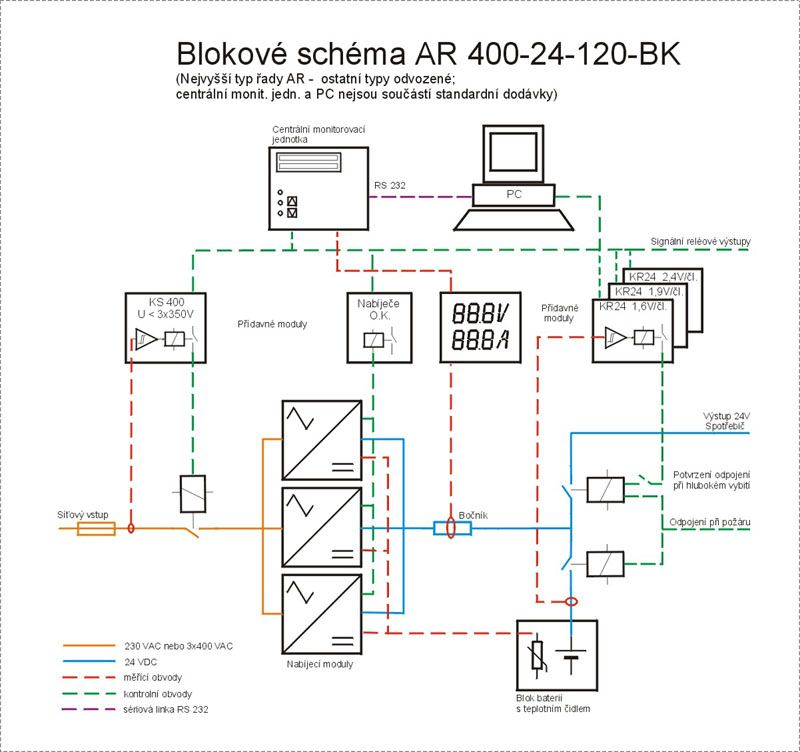
\includegraphics[width=0.7\textwidth]{fig/blokove_schema.png}
    \caption{Blokové schéma napájecího systému a integrace jednotky do pracoviště}
    \label{fig:blokove_schema}
\end{figure}

Vývojový hardwarový prototyp řídicí desky, na kterém probíhalo experimentální testování a ladění senzorických rozhraní, je zachycen na fotografii na obrázku~\ref{fig:prototyp_desky}.

\begin{figure}[htbp]
    \centering
    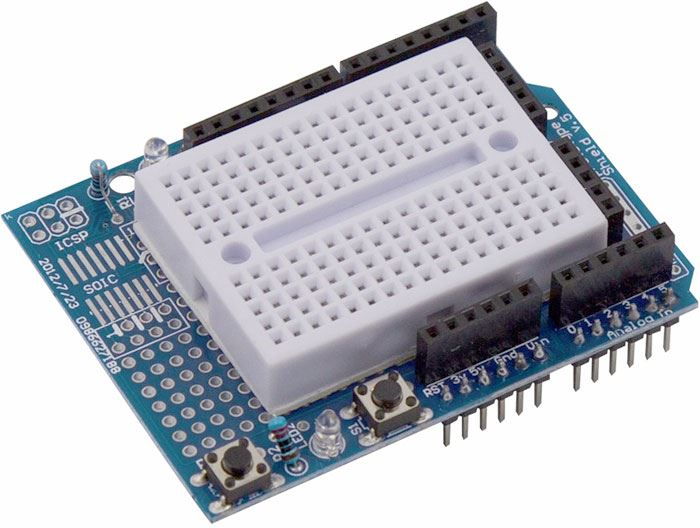
\includegraphics[width=0.7\textwidth]{fig/prototyp_desky.jpg}
    \caption{Prototypová vývojová deska s nepájivým polem pro testování obvodů}
    \label{fig:prototyp_desky}
\end{figure}

Mezi hlavní podsystémy monitorovací stanice patří tyto moduly:
\begin{enumerate}
    \item \textbf{Napájecí část} – zajišťuje filtraci a stabilizaci napětí na hodnotu $3,3\,\mathrm{V}$ z průmyslového rozvodu $24\,\mathrm{V}$.
    \item \textbf{Senzorické rozhraní} – obsahuje analogově-digitální převodníky pro vyhodnocení napěťových úrovní.
    \item \textbf{Komunikační modul} – realizuje fyzickou vrstvu sběrnice pro odesílání dat.
\end{enumerate}

\section{Senzorické pole a typografická pravidla měření}
Pro ověření funkčnosti byly k jednotce připojeny senzory teploty a tlaku. Při kalibraci bylo dosaženo optimálních výsledků v teplotním rozsahu od $-20\,^{\circ}\mathrm{C}$ do $85\,^{\circ}\mathrm{C}$. Maximální provozní tlak v testovací komoře dosahoval hodnoty $p_{max} = 1,5\,\mathrm{MPa}$ při konstantním průtoku $Q = 2,4\,\mathrm{l\cdot min^{-1}}$. 

Při zpracování naměřených hodnot v textu je nutné striktně dodržovat pravidla české technické typografie. Číselné údaje a jejich jednotky musí být vždy odděleny nezlomitelnou mezerou (např. v~textu psáno jako \texttt{24\textasciitilde mA}, v \LaTeX{}u ošetřeno pomocí vlnovky nebo úzké mezery \texttt{\textbackslash,}), aby nedošlo k~jejich zalomení na nový řádek.

\chapter{Realizace a naměřené výsledky}
V rámci experimentálního testování byla sledována odezva systému při skokové změně zátěže. Měření probíhalo po dobu $t = 120\,\mathrm{s}$ s periodou vzorkování $T = 10\,\mathrm{ms}$.

\section{Analýza spotřeby a frekvenční charakteristiky}
Důležitým parametrem vestavěných zařízení je jejich proudový odběr v různých provozních režimech. Výsledky měření spotřeby v závislosti na taktovací frekvenci mikrokontroléru jsou přehledně uspořádány v~tabulce~\ref{tab:spotreba_mcu}.

\begin{table}[htbp]
    \centering
    \caption{Závislost proudového odběru na frekvenci jádra}
    \label{tab:spotreba_mcu}
    \begin{tabular}{|c|c|c|c|}
        \hline
        \textbf{Index měření} & \textbf{Frekvence [MHz]} & \textbf{Napětí [V]} & \textbf{Odběr [mA]} \\ \hline
        1 & 8  & 3,3 & 4,2  \\ \hline
        2 & 16 & 3,3 & 7,8  \\ \hline
        3 & 48 & 3,3 & 18,5 \\ \hline
        4 & 96 & 3,3 & 35,1 \\ \hline
    \end{tabular}
\end{table}

Kromě analýzy napájení byla v rámci podsystému senzorického rozhraní zkoumána frekvenční závislost vstupního analogového filtru, který potlačuje vysokofrekvenční rušení před převodem signálu. Naměřená amplitudová charakteristika tohoto RC filtru s rezistorem $R = 150\,\Omega$ a kapacitou $C = 1\,\mu\mathrm{F}$ je zobrazena na obrázku~\ref{fig:graf_filtru}. Mezní kmitočet filtru činí teoreticky i prakticky $f_0 = 1023\,\mathrm{Hz}$ při poklesu zisku o $-3\,\mathrm{dB}$.

\begin{figure}[htbp]
    \centering
    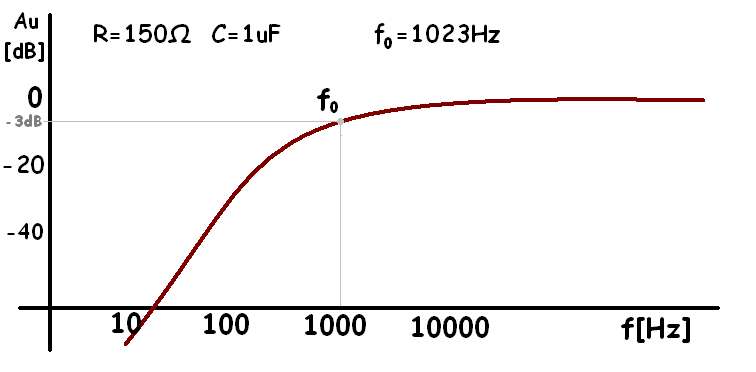
\includegraphics[width=0.7\textwidth]{fig/graf_spotreby.jpg}
    \caption{Amplitudová frekvenční charakteristika analogového RC filtru}
    \label{fig:graf_filtru}
\end{figure}


Pro teoretický výpočet celkového elektrického příkonu $P$ střídavých podsystémů monitoru se využívá vztah:
\begin{equation}
P = U \cdot I \cdot \cos\varphi
\label{eq:vykon}
\end{equation}
kde $U$ je efektivní napětí, $I$ je procházející proud a $\cos\varphi$ představuje účiník.

\section{Programová implementace}
Základní inicializace a vyčítání dat ze sběrnice jsou realizovány nízkoúrovňovým algoritmem v~jazyce C. Ukázka zdrojového kódu, který konfiguruje interní registr analogově-digitálního převodníku (ADC), je uvedena v~příkladu~\ref{lst:kod_adc}.

\begin{lstlisting}[language=C, caption={Konfigurace a inicializace ADC registru}, label={lst:kod_adc}, frame=single]
#include <stdint.h>

#define ADC_CR_REG  (*((volatile uint32_t*)0x40012000))
#define ADC_ENABLE  (1 << 0)

void init_adc_peripheral(void) {
    // Zapnuti periferie ADC pomoci prislusneho bitu
    ADC_CR_REG |= ADC_ENABLE;
    
    /* Cekani na stabilizaci referencniho napeti */
    for(volatile int i = 0; i < 1000; i++);
}
\end{lstlisting}

Jak je zřejmé z~ukázky kódu~\ref{lst:kod_adc}, registry jsou mapovány přímo do paměťového prostoru mikrokontroléru. Na nízkoúrovňovou konfiguraci navazuje obslužná funkce pro samotné vyčítání dat z převodníku, jejíž implementace je uvedena v~příkladu~\ref{lst:read_data}.

\begin{lstlisting}[language=C, caption={Funkce pro vyčítání dat z převodníku}, label={lst:read_data}, frame=single]
uint16_t read_adc_data(void) {
    // Spusteni konverze a cekani na dokonceni
    ADC_CR_REG |= (1 << 2); 
    while(!(ADC_CR_REG & (1 << 4)));
    
    // Navraceni vysledne hodnoty z datoveho registru
    return (uint16_t)(*((volatile uint32_t*)0x40012004));
}
\end{lstlisting}

Tato modulární struktura zajišťuje maximální rychlost odezvy, která je v~průmyslových aplikacích kritická.

\chapter*{Závěr}
\addcontentsline{toc}{chapter}{Závěr}

V rámci této semestrální práce byl úspěšně navržen a implementován funkční prototyp modulární monitorovací jednotky určené pro sběr fyzikálních veličin v náročném průmyslovém prostředí. Cíle stanovené v úvodu práce byly kompletně splněny.

Během realizace byla úspěšně ověřena integrace senzorických polí a hardwarová architektura založená na 32bitovém mikrokontroléru s jádrem ARM Cortex-M4. Experimentální měření proudového odběru v závislosti na taktovací frekvenci potvrdilo lineární nárůst spotřeby a ukázalo na nutnost implementace dynamického managementu napájení pro úsporné průmyslové režimy. Dále byla úspěšně nasazena analogová filtrace šumu pomocí RC filtru, u kterého byla ověřena teoretická i praktická frekvenční charakteristika s mezním kmitočtem $f_0 = 1023\,\mathrm{Hz}$.

Z hlediska softwarové vrstvy byla vytvořena modulární, nízkoúrovňová implementace v jazyce C, která díky přímému mapování registrů do paměťového prostoru zajišťuje minimální latenci při vyčítání dat. Celý ukázkový dokument i doprovodná prezentace byly zpracovány v typografickém systému \LaTeX\ za přísného dodržení pravidel české technické typografie a specifických směrnic Technické univerzity v Liberci.
%\nocite{*}
% Aplikace biblatexu a stylu citování ČSN ISO 690, 
% soubor refPsaniTextuNEW.bib je vložen v hlavičce dokumentu

\printbibliography[title={Použitá literatura},heading=bibintoc] % sazba seznamu citací a vložení do obsahu 
% \printbibliography[title={References},heading=bibintoc] 

% \addcontentsline{toc}{chapter}{References} 
%%%%%%%%%%%%%%%%%%%%%%%%%%%%%%%%%%%%%%%%%%%%%%%%%%%%%%%%%%%%%%%%%%%%%%%%%%%%%%%%%%


\renewcommand{\indexname}{Přehled příkazů, prostředí a voleb}
\printindex

\appendix % začátek příloh / beginning of appendiecies
\chapter{Přílohy}
\section{Obsah vloženého balíku do IS/STAG TUL} % příklad přílohy 
\begin{itemize}
    \item Text práce
    \item Obrazová dokumentace
    \item Zdrojové kódy
    \item \dots
\end{itemize}

\section{Velké tabulky a obrázky} % příklad přílohy 

\end{document}
